\documentclass[border=2pt]{standalone}
\usepackage{tikz}
\usepackage{amsmath}
\usepackage{mathtools}
\usepackage{adjustbox}
\usetikzlibrary{patterns}
\usetikzlibrary{calc} \usetikzlibrary{positioning} \usetikzlibrary{shapes,arrows} \usetikzlibrary{plotmarks}
\usetikzlibrary{positioning,decorations.pathreplacing}
\tikzset{
itria/.style={
  draw,dashed,shape border uses incircle,
  isosceles triangle,shape border rotate=90,yshift=-0.8cm}
}

\begin{document}

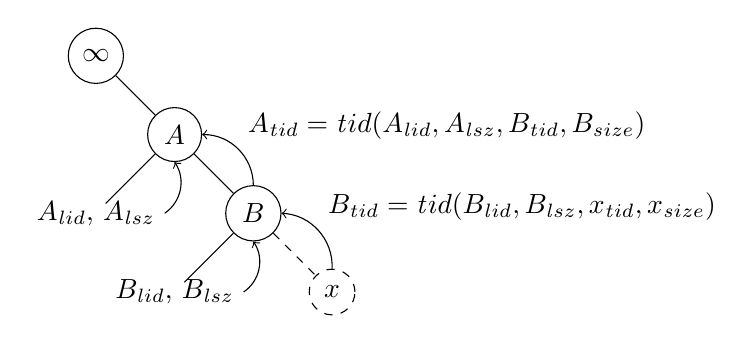
\begin{tikzpicture}[level/.style={sibling distance=20mm, level distance=10mm},baseline=(inf.base)]
\node [circle,draw](inf){$\infty$}
  child[missing]{}
  child { node[circle,draw](Atid){$A$}
    child { node[]{}
            { node[](Alsub){$A_{\mathit lid}$, $A_{\mathit lsz}$}}
    }
    child { node[circle,draw](Btid){$B$}
      child { node[]{}
            { node[](Blsub){$B_{\mathit lid}$, $B_{\mathit lsz}$}}
      }
      child[dashed] { node[circle,draw](xtid){$x$}
        child[missing]{}
        child[missing]{}
      }
    }
  };

\path[solid,->](Alsub)edge [bend right=45]  (Atid);
\path[solid,->](Btid)edge [bend right=45] node[above right]{$A_{\mathit tid}={\mathit tid}(A_{\mathit lid}, A_{\mathit lsz}, B_{\mathit tid}, B_{\mathit size})$} (Atid);
\path[solid,->](Blsub)edge [bend right=45]  (Btid);
\path[solid,->](xtid)edge [bend right=45] node[above right]{$B_{\mathit tid}={\mathit tid}(B_{\mathit lid}, B_{\mathit lsz}, x_{\mathit tid}, x_{\mathit size})$} (Btid);
\end{tikzpicture}

\end{document}